\documentclass[11pt]{article}

\usepackage[margin=1in]{geometry}
\usepackage[T1]{fontenc}
\usepackage[utf8]{inputenc}
\usepackage{csquotes}

\usepackage[backend=biber,style=numeric,sorting=none,maxnames=3,minnames=1]{biblatex}
\addbibresource{refs.bib}

\usepackage{hyperref}

\usepackage{bucket}

\hypersetup{
  colorlinks = true,
  linkcolor  = bucketblue,
  citecolor  = bucketblue,
  urlcolor   = bucketblue,
}

\newcommand{\emp}[1]{\textcolor{bucketgray}{\footnotesize [empirical: #1]}}
\newcommand{\hai}{\emp{packages/bkt/src/hai, 2026-10-07, git show dev:packages/bkt/src/hai}}
\newcommand{\bank}{\emp{packages/bkt/hai/bank.json and review.json, 2026-10-07, bkt hai freeze; bkt hai review}}
\newcommand{\calc}{\emp{packages/bkt/src/hai/stats.ts halfWidthItems, 2026-10-07, evaluated by hand}}

\glossentry{hp}{unaided score}%
  {https://github.com/gianyrox/bucket-foundation/blob/dev/packages/bkt/src/hai/stats.ts}%
  {$H_p$, the guess-corrected share of solo items a person gets right with no AI answer shown; see \Cref{def:scores}.}
\glossentry{a}{AI score}%
  {https://github.com/gianyrox/bucket-foundation/blob/dev/packages/bkt/src/hai/score.ts}%
  {$A$, the guess-corrected share of the same frozen items the model gets right on its own; see \Cref{def:scores}.}
\glossentry{jp}{joint score}%
  {https://github.com/gianyrox/bucket-foundation/blob/dev/packages/bkt/src/hai/stats.ts}%
  {$J_p$, the guess-corrected share of pair items a person gets right after the model's answer and rationale are shown; see \Cref{def:scores}.}
\glossentry{mp}{multiplier}%
  {https://github.com/gianyrox/bucket-foundation/blob/dev/packages/bkt/src/hai/stats.ts}%
  {$m_p = J_p / \max(H_p, A)$, the joint score over the better single agent; see \Cref{def:multiplier}.}
\glossentry{rp}{retention}%
  {https://github.com/gianyrox/bucket-foundation/blob/dev/packages/bkt/src/hai/stats.ts}%
  {$R_p = H_p(t + 7\,\mathrm{d}) - H_p(t)$, the change in the unaided score on the same items after seven days; see \Cref{def:retention}.}
\glossentry{dependence}{dependence}%
  {https://github.com/gianyrox/bucket-foundation/blob/dev/packages/bkt/src/hai/stats.ts}%
  {The state in which a tool raises the joint score while the person keeps none of the gain a week later; see \Cref{def:dependence}.}
\glossentry{probe}{probe}%
  {https://github.com/gianyrox/bucket-foundation/blob/dev/packages/bkt/src/hai/probe.ts}%
  {One session of 40 unseen items in 20 matched pairs, one item of each pair solo and one with AI, retested unaided seven days later; see \Cref{def:probe}.}

\title{Human-AI-Computer Interaction: Measuring Whether AI Strengthens Unaided Judgment}
\author{Gianangelo Dichio\\Bucket Foundation}
\date{2026-10-07}

\begin{document}
\maketitle

\begin{abstract}
A tool that helps a person answer today and leaves them no better at answering alone next week has made them dependent on it. We state a measurement protocol that separates the two outcomes. On one task set, three scores are taken: the person's \term{hp}{unaided score} $H_p$, the model's \term{a}{AI score} $A$, and the person's \term{jp}{joint score} $J_p$ with the model's answer in view. The \term{mp}{multiplier} is $m_p = J_p / \max(H_p, A)$, the gain is $D = J_p - \max(H_p, A)$, and the unaided test is repeated after seven days to give \term{rp}{retention} $R_p = H_p(t + 7\,\mathrm{d}) - H_p(t)$ and learning $L = J_p(t + 7\,\mathrm{d}) - H_p(t + 7\,\mathrm{d})$. A tool that raises $J_p$ while $L$ stays at or below zero across its interval marks \term{dependence}{dependence}. The instrument is the \texttt{hai} probe in Bucket's \texttt{bkt} package: a frozen bank of 998 four-choice items across the seven canon branches, of which 68 are held out by an automated distractor review \bank; sessions of 40 items in 20 pairs matched on tier and on whether the model got the pair's items right; a 20 second think window before the model's answer appears; no feedback until the retest; guess-corrected scores and a bootstrap over pairs for every interval \hai. The instrument is built and no probe has been retested, so this report carries no result. It states the planned analysis, paired comparisons stratified by education level, a divergence hypothesis on how reliance on one model narrows the range of answers across a group, and the rule by which the scores decide which tasks Research OS hands to the model and which it keeps with the person.
\end{abstract}

\section{Introduction}
\label{sec:intro}

Research OS puts a model next to a person on every task in the product: recall of a result, application of a rule, derivation, teaching. Each of those tasks can be left with the person, augmented with the model, or handed to the model. The product has no basis for that choice until it can measure, per person and per task class, what the model adds today and what the person keeps a week later. Field studies report the first number, the lift with the model in hand \autocite{dellacqua2023jagged,brynjolfsson2023generative}, and a meta-analysis across 106 experiments finds that human and AI together score below the better of the two on average \autocite{vaccaro2024combinations}. The second number, what the person retains, is the one a learning product cannot do without: in a randomized study of high school mathematics, access to a model raised practice scores and lowered unaided exam scores \autocite{bastani2025guardrails}. This report defines both numbers on the same items, describes the instrument that takes them, and says what will be done with them.

\section{Related work}
\label{sec:related}

Complementary team performance, the case where the pair beats both the person and the model, was named and tested in a user study of AI explanations, which found explanations raised acceptance of the model's answer whether it was right or wrong \autocite{bansal2021whole}. The jagged frontier study randomized consultants to model access and found gains inside the model's competence and losses outside it \autocite{dellacqua2023jagged}; the customer-support study found the largest gains for the least experienced workers \autocite{brynjolfsson2023generative}. The retention arm of this protocol follows the testing-effect literature, in which an unaided retrieval test is itself the strongest predictor of later recall \autocite{roediger2006testing}. The divergence hypothesis of \Cref{sec:divergence} follows a study in which model assistance raised the rated quality of each writer's story and lowered the diversity across writers \autocite{doshi2024diversity}. Intervals use the pair bootstrap \autocite{efron1979bootstrap}.

\section{Preliminaries}
\label{sec:prelim}

\begin{definition}[Item and bank]
\label{def:bank}
An item is a prompt with four choices, one correct, drawn from the Academy pack and frozen with three distractors fixed under a seed, so the same text is shown to every person and to the model. The bank is versioned by a hash of its items \hai. An automated review flags an item whose distractors duplicate each other, contain or overlap the answer by token Jaccard at or above 0.5, answer a second question on the same atom, or whose answer runs to at least twice the length of its longest distractor; a flagged item stays out of probes and scoring until a person clears it \hai.
\end{definition}

\begin{definition}[Scores]
\label{def:scores}
For $c$ correct answers out of $n$ four-choice items, the guess-corrected score is $s = (c/n - 1/4)/(3/4)$, so chance scores 0 and a perfect run scores 1 \hai. The \term{hp}{unaided score} $H_p$ is $s$ over a person's solo items; the \term{jp}{joint score} $J_p$ is $s$ over their pair items; the \term{a}{AI score} $A$ is $s$ for the model over those same pair items.
\end{definition}

\begin{definition}[Probe]
\label{def:probe}
A \term{probe}{probe} is 40 unseen bank items in 20 pairs. Items are grouped by tier and by whether the model got them right, pairs are drawn inside a group, and a seeded coin sends one item of each pair to the solo condition and the other to the pair condition \hai. In the pair condition the model's choice and a rationale of at most 25 words appear after 20 seconds; the person may accept or override, and the acceptance is recorded \hai. No correctness is shown on any probe item, and probe items never enter spaced review, until the retest ends \hai.
\end{definition}

\begin{definition}[Retest]
\label{def:retest}
Seven days after a probe, the person answers all 40 of its items again, unaided, in a reshuffled order \hai. Scores and answers appear only after the retest.
\end{definition}

\begin{definition}[Multiplier and gain]
\label{def:multiplier}
The \term{mp}{multiplier} is $m_p = J_p / \max(H_p, A)$, reported as null when $\max(H_p, A) < 0.1$; the gain is $D = J_p - \max(H_p, A)$ \hai. $D$ is the primary statistic and $m_p$ is reported beside it.
\end{definition}

\begin{definition}[Retention and learning]
\label{def:retention}
\term{rp}{Retention} is $R_p = H_p(t + 7\,\mathrm{d}) - H_p(t)$ over the solo items. Learning is $L = J_p(t + 7\,\mathrm{d}) - H_p(t + 7\,\mathrm{d})$: at the retest, the score on items first seen with the model minus the score on items first seen alone, both unaided \hai.
\end{definition}

\begin{definition}[Dependence]
\label{def:dependence}
\term{dependence}{Dependence} is flagged when the 95\% interval of $J_p - H_p$ lies above zero and the 95\% interval of $L$ includes or lies below zero \hai. The gain was there with the model in the room and gone a week later.
\end{definition}

\section{Method}
\label{sec:method}

\begin{figure}[htbp]
  \centering
  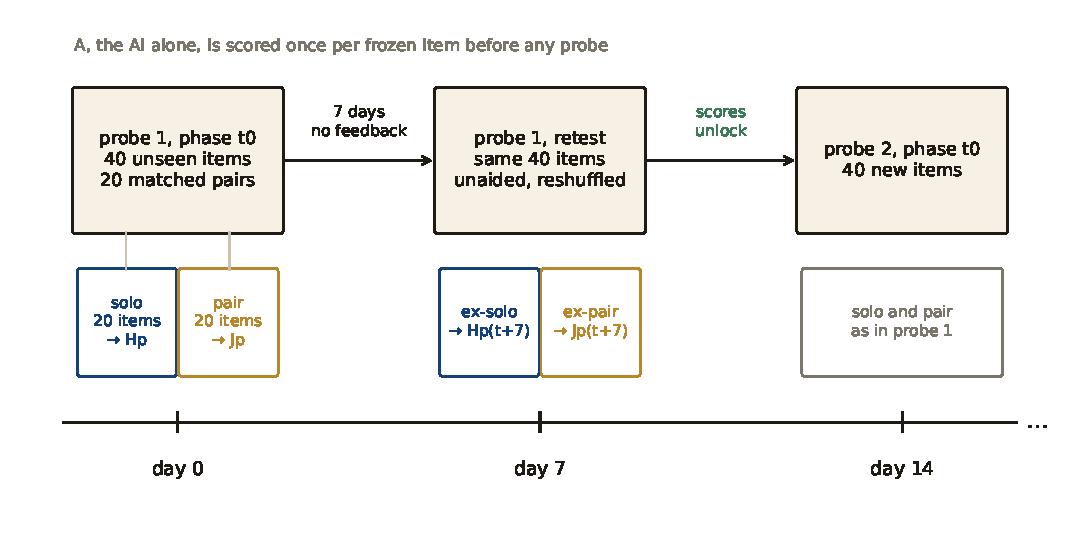
\includegraphics[width=\linewidth]{figures/fig_timeline.pdf}
  \caption{The session timeline. Each probe splits 40 unseen items into solo and pair conditions on day 0, is retested unaided in full on day 7, and unlocks its scores only then; the next probe draws 40 new items. $A$ is scored on every frozen item once, before any person sees it.}
  \label{fig:timeline}
\end{figure}

\begin{figure}[htbp]
  \centering
  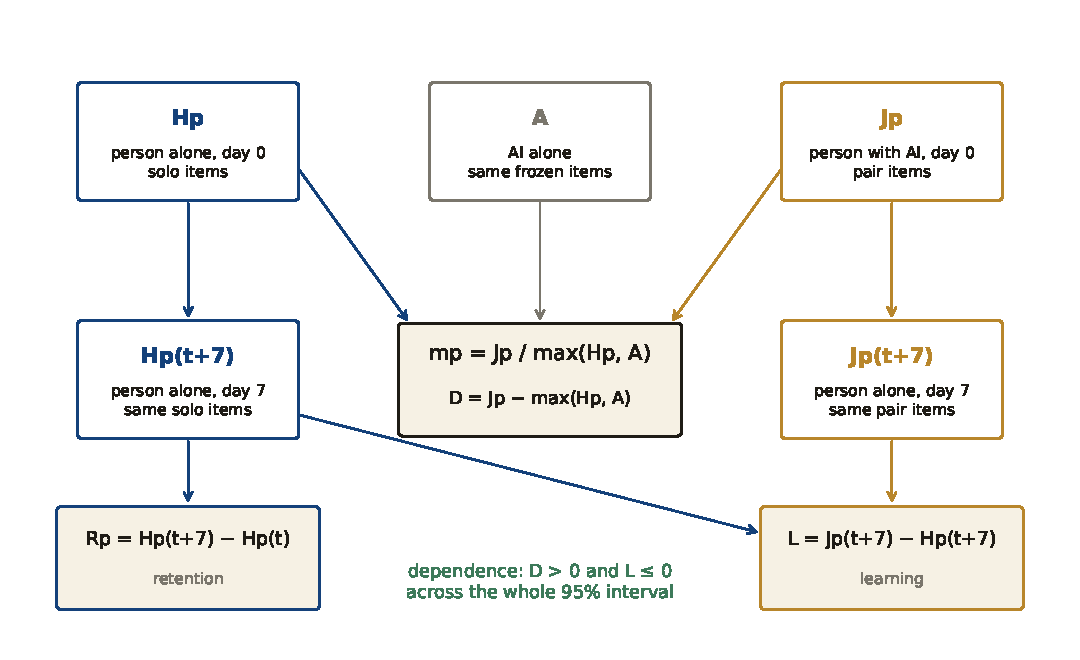
\includegraphics[width=0.92\linewidth]{figures/fig_scores.pdf}
  \caption{The four scores and the statistics derived from them. $H_p$, $A$ and $J_p$ combine into the multiplier and the gain; the day 7 scores give retention on the solo items and learning on the pair items; dependence is the pattern where the gain is positive and learning is not.}
  \label{fig:scores}
\end{figure}

\paragraph{The instrument.}
The probe lives in \texttt{packages/bkt/src/hai/} and runs inside the \texttt{bkt} terminal app, offline, with answers sealed in the same encrypted store as the person's other attempts; nothing leaves the device, and the person can export or wipe their data \hai. \texttt{bkt hai freeze} writes the bank, \texttt{bkt hai review} writes the flags, \texttt{bkt hai score} sends the bank to the model through a batch job and stores each answer with its rationale, model id and date, \texttt{bkt hai} runs a probe or its retest, and \texttt{bkt hai report} prints the scores as sentences \hai.

\paragraph{The AI condition.}
$A$ is one run of \texttt{claude-opus-5-5} at low effort over each frozen item, the reply constrained to a JSON object holding a letter and a rationale, with 400 output tokens at most \hai. A reply that fails to parse, names no valid letter or hits the token cap is counted as malformed and left out of $A$ and of pair matching \hai. The model sees the same four choices the person sees, so $A$ is a property of the item and the bank version.

\paragraph{Matching.}
Pairs are matched on tier and on the model's correctness so that $H_p$ and $J_p$ are taken on items of the same difficulty and the same model behaviour. A matched pair in which the model is wrong measures whether the person overrides it; a pair in which it is right measures whether they accept it.

\paragraph{Intervals.}
Every interval is a 95\% percentile bootstrap over matched pairs, 2,000 draws under a fixed seed, resampling pairs and keeping both items of each \hai. An interval is withheld when fewer than half the draws yield a finite statistic \hai. For a half-width of 0.10 on $J_p - H_p$ at a true score near 0.5, the guess-corrected scale needs about 342 items per condition; a half-width of 0.15 needs about 152 \calc. The 998-item bank caps one person at 499 items per condition \bank, so the design target is a half-width of 0.10 after 17 probes, and no trend is shown before 5 retested probes \hai.

\section{Design}
\label{sec:design}

\subsection{Status}
\label{sec:status}

The bank is frozen at 998 items: 482 recall, 240 apply, 177 derive, 90 teach and 9 conceptual, across biophysics (281), information (120), mind (120), cosmology (118), mathematics (110), physics (110), chemistry (110) and learning-to-learn (29) \bank. The review flags 68 items and none has been cleared \bank. No AI scores have been collected, no probe has been run, and \texttt{bkt hai report} prints that no probe has been retested \bank. Every number above is a property of the instrument or a planning quantity. There are no values of $H_p$, $A$, $J_p$, $m_p$, $R_p$ or $L$ to report.

\subsection{Planned analysis}
\label{sec:analysis}

Per person, the report is $D$ with its interval, $m_p$ beside it, $R_p$, $L$ and the dependence flag, each with the number of pairs behind it, and the number of malformed model replies left out. Within a person, $D$ and $L$ are also broken out by tier and by whether the model was right on the pair, so a positive $D$ driven by accepting correct answers is told apart from one driven by overriding wrong ones.

Across people, every comparison is paired: each person contributes their own $H_p$, $J_p$ and retest scores on their own matched items, and the group statistic is the mean of the per-person differences with a bootstrap over people. Participants are stratified by highest education level reported at consent, in four bands: secondary, bachelor's, master's, doctoral. The question for the strata is whether $D$ and $L$ move together or apart with prior training, since the field studies cited above found the largest lift for the least experienced \autocite{brynjolfsson2023generative} and the learning study found that unaided exam scores fell where the model gave answers and held where it gave hints \autocite{bastani2025guardrails}. The education band is stored at consent and nowhere else, and a band with fewer than 20 people reports counts only.

\subsection{The divergence hypothesis}
\label{sec:divergence}

The hypothesis is that a group of people answering with the same model converges on the model's answers and the model's phrasings, so the range of ideas the group produces narrows even where each person's score rises. Four-choice items cannot show this, since the answer space is fixed, so the test needs open items: a second bank of short free-response prompts in the derive and teach tiers, each with a rubric. Each person answers a matched half alone and a half with the model's draft in view. The responses are embedded with the same sentence encoder Bucket uses for the solvability atlas, and divergence is measured as the mean pairwise cosine distance among the group's answers to one prompt, solo against pair, with a bootstrap over people. A second measure is the number of distinct answer clusters at a fixed distance threshold. The prediction, following \textcite{doshi2024diversity}, is a higher rubric score and a lower pairwise distance in the pair condition. A product that raises every person's score while collapsing the group's spread has optimized the wrong thing for a research community, whose value is in the answers nobody else gave.

\subsection{Decision rule for Research OS}
\label{sec:decision}

The scores decide, per task class, what Research OS does with the model. \Cref{tab:decision} gives the rule. A class where $D$ is above zero and $L$ is at or above zero is augmented: the model's answer stays in view and the person's own attempt stays first. A class where $D$ is above zero and $L$ is below zero, the dependence pattern, is augmented only when the task is a means and never when it is a learning target; in the Learn module it falls back to unaided practice with the model held until after the attempt. A class where $D$ is at or below zero is left with the person. A class where $A$ exceeds $H_p$ and $J_p$ sits at $A$ is a candidate for replacement, meaning the model answers and the person reviews, and only outside the Learn module. The rule is applied per person, since the same class can fall in different cells for different people, and the cells are re-read after each retested probe.

\begin{table}[htbp]
  \centering
  \caption{What Research OS does with a task class, by the signs of the gain and of learning.}
  \label{tab:decision}
  \begin{tabular}{@{}lll@{}}
    \toprule
    Gain $D$ & Learning $L$ & Action \\
    \midrule
    $> 0$ & $\geq 0$ & augment: model answer in view after the person's attempt \\
    $> 0$ & $< 0$ & augment as a means only; unaided in Learn \\
    $\leq 0$ & any & leave with the person \\
    $A > H_p$, $J_p \approx A$ & any & candidate to replace outside Learn; person reviews \\
    \bottomrule
  \end{tabular}
\end{table}

\section{Calibration}
\label{sec:calibration}

The central claims are the definitions, and their calibration is the instrument's test suite and the Lean listing. The tests check that the freeze is deterministic across builds, that pairs match on tier and model correctness, the guess correction at chance and at a perfect run, the four statistics on fixed data, the pair bootstrap on fixed data under a fixed seed, that no feedback is shown before the retest, and that the retest is gated by an injected clock \hai. \Cref{app:lean} checks that the retest time is after the probe time, that the guess-corrected numerator lies between the negative item count and the denominator for any count of correct answers at most the item count, that it is zero at chance, and that the dependence flag requires a positive gain and cannot fire when learning is positive. The error budget on a reported statistic is its bootstrap interval, and \Cref{sec:method} gives the item counts that interval needs.

\section{Limitations}
\label{sec:limitations}

\paragraph{No data.}
No probe has been retested, so nothing here has been measured on a person. The bank, the matching and the statistics have been exercised by tests on fixed data only.

\paragraph{One model, one run.}
$A$ is one run of one model at one effort setting. A different model, a higher effort or a second sample would give a different $A$ and a different pairing. The bank version and the model id are stored with every score so that a re-run is a new instrument version and never a silent change.

\paragraph{Four-choice items.}
The bank measures recognition under four fixed choices. It cannot show divergence, and it rewards a model that is good at eliminating distractors. The open-item bank of \Cref{sec:divergence} is unbuilt.

\paragraph{Seven days.}
The retest interval is fixed at seven days. Retention at thirty days or ninety is a different quantity, and a single interval cannot separate forgetting from a spacing effect.

\paragraph{Self-selection and the flagged items.}
Participants are users of a terminal app who opt in; the education strata will reflect that. The 68 flagged items are out until a person clears them, and the automated review is a set of surface rules, so an item with a subtler cue can pass it.

\paragraph{The decision rule.}
\Cref{tab:decision} is a rule with no result behind it yet. Its cells are set by the signs of two statistics and say nothing about effect size; a positive $D$ of 0.02 and one of 0.30 fall in the same cell. Thresholds on size wait for the first intervals.

\paragraph{Licences.}
The item bank is derived from the Academy pack, whose lesson text is open and whose sources are listed per atom in the pack; the probe code is MIT with the repository. Per-person data never leaves the device, and the planned cross-person analysis uses only exported, consented records.

\printbibliography

\appendix

\section{Glossary}
\label{app:glossary}

\printglossaryentry{hp}
\printglossaryentry{a}
\printglossaryentry{jp}
\printglossaryentry{mp}
\printglossaryentry{rp}
\printglossaryentry{dependence}
\printglossaryentry{probe}

\section{Lean listings}
\label{app:lean}

\texttt{lean/Bucket/Multiplier.lean}, checked by \texttt{make lean}, holds the four facts the method leans on. The guess-corrected score is carried as an integer numerator $4c - n$ over the denominator $3n$.

\begin{lstlisting}[style=bucketlean]
def RETEST_MS : Nat := 7 * 24 * 60 * 60 * 1000
def retestDue (t : Nat) : Nat := t + RETEST_MS
theorem retestDue_gt (t : Nat) : t < retestDue t

structure Probe where
  correct : Nat
  items : Nat
  bounded : correct <= items

def Probe.numerator (p : Probe) : Int := 4 * (p.correct : Int) - p.items
def Probe.denominator (p : Probe) : Int := 3 * (p.items : Int)
theorem Probe.numerator_le_denominator (p : Probe) : p.numerator <= p.denominator
theorem Probe.numerator_ge_neg_items (p : Probe) : -(p.items : Int) <= p.numerator
theorem Probe.numerator_zero_at_chance (p : Probe) (h : 4 * p.correct = p.items) :
    p.numerator = 0

structure Interval where
  lo : Int
  hi : Int

def dependence (gain learning : Interval) : Prop := 0 < gain.lo /\ learning.lo <= 0
theorem dependence_needs_gain (gain learning : Interval) (h : dependence gain learning) :
    0 < gain.lo
theorem no_dependence_when_learning_kept (gain learning : Interval) (h : 0 < learning.lo) :
    ~ dependence gain learning
\end{lstlisting}

\texttt{lake build} output, quoted verbatim \emp{papers/human-ai-multiplier/lean, 2026-10-07, make lean}.
% voice-ignore-next 3
\begin{verbatim}
Build completed successfully (4 jobs).
\end{verbatim}

\end{document}
